% Preamble
\documentclass[a4paper, 12pt]{article}
\usepackage[margin=1in]{geometry} % Set margin
\usepackage{pdfpages} % Insert pdf pages
\usepackage{amssymb,amsmath,amsthm, amsfonts} % Math libraries

% Custom commands
\newcommand{\sub}[1]{\subsection{\underline{#1}}}
\newcommand{\subsub}[1]{\subsubsection{\underline{#1}}}
\newcommand{\?}{\stackrel{?}{=}}
\newcommand{\R}{\ensuremath{\mathbb{R}}}
\newcommand{\F}{\ensuremath{\mathbb{F}}}
\newcommand{\eqbcuz}[1]{\text{~$\stackrel{(#1)}{=}$~}}
\renewcommand{\qed}{$$\blacksquare$$}
\renewcommand{\b}[1]{\textbf{#1}}
\renewcommand{\because}[1]{~\b{(#1)}\\}
\renewcommand{\d}{\ensuremath{\Downarrow\\~}}

% Begin Document %
\begin{document}

% Title Page
\begin{titlepage}
    %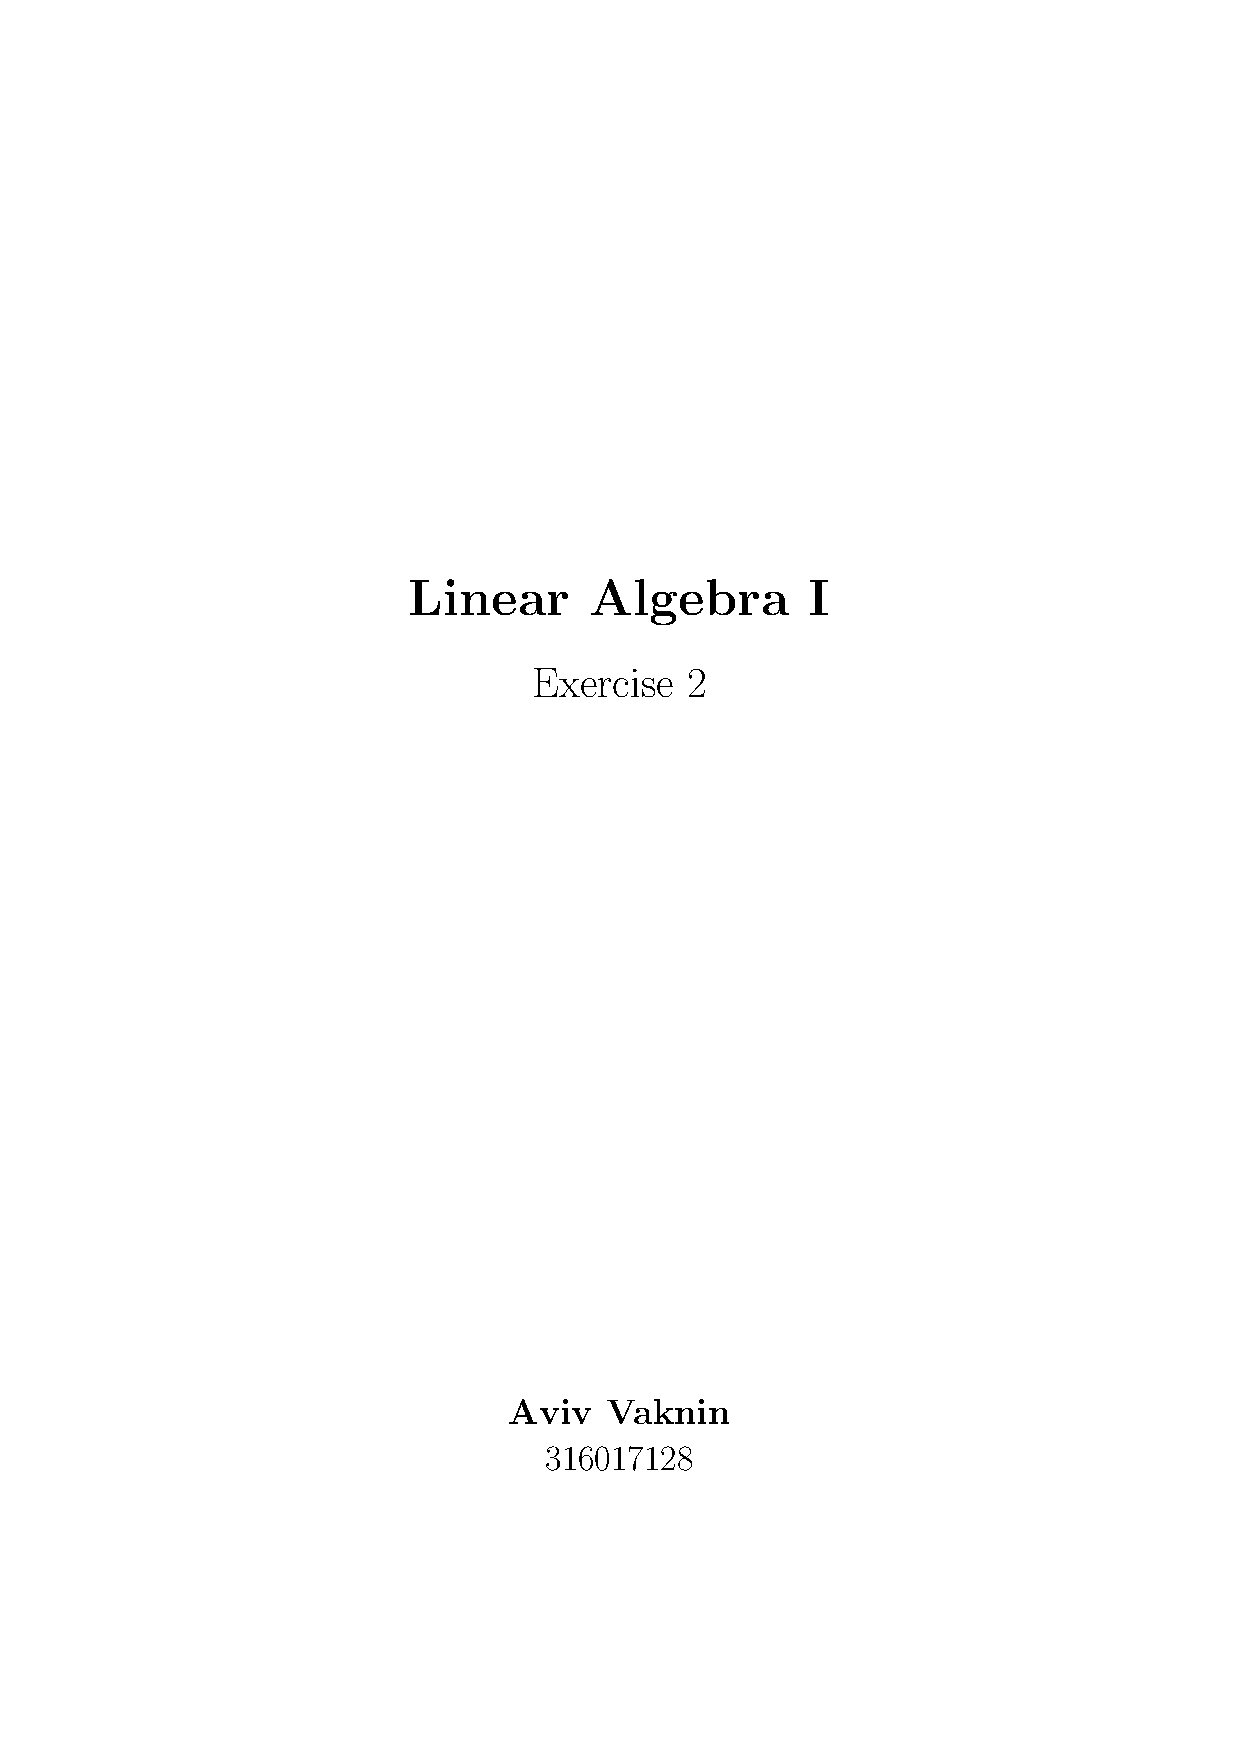
\includepdf{title.pdf}
\end{titlepage}

% 7
\setcounter{section}{6}
\section{Find the solution set for: $$X+Y-Z=-1$$ $$X-Y-Z=-1$$}
First, let's isolate $X$:
$$ X=Z-Y-1 $$
$$ X=Z+Y-1 $$
From the above, we can conclude that $Y=0$.
If we change one of the original equations, we'll get: $$ X=Z-1 $$
Therefore, the solution set for $X,Y,Z$ is:
$$
S = \Bigg{\{}
    \bordermatrix {
    &        \cr
    & z-1    \cr
    & y    \cr
    & z    \cr
    }
:
y, z \in {\R}
\Bigg{\}}
$$
\qed

% 8
\section{Show that the inverse of the inheritance rule is not true.}
The equations system:
$$ x^1 + x^2 = 1 $$
$$ x^2 - x^3 = 3 $$

We can generate the equation $L$, which is a linear form of the mentioned two equations,
by multiplying the first equation by $3$, and the second one by $(-1).$
$$ L: 3x^1 + 2x^2 + x^3 = 0 $$

As we can easily see, the following solution to $L$ is not a solution to the equations system:
$$ x^1=0 $$ $$ x^2=0 $$ $$ x^3=0 $$
\qed\pagebreak

% 10
\setcounter{section}{9}
\section{Are the two equation systems equivalent? if yes, write every equation as a linear form of the other system.}
\sub{Showing the systems are equivalent}
\subsub{Right-hand side system}
First, let's find the solutions set of the right-hand side system.\\
We can easily see from the first equation that $X^1=X^3$, in addition, let's declare $t^1=X^3$.\\
Now, from the second equation, we get: $$ X^2 = -3t^1 $$
This leads us to the following solutions set for the right-hand side system:
$$
S = \Bigg{\{}
    \bordermatrix {
    &        \cr
    & t^1    \cr
    & -3t^1    \cr
    & t^1    \cr
    }
:
t^1 \in {\R}
\Bigg{\}}
$$

\subsub{Left-hand side system}
Let's find the linear form of $L_2-2L_3$: $$ X^2+3x^3 = 0 $$
Which leads us to: $$ X^2 = -3x^3 $$
In addition, we'll mark $X^3$ as $t^1$, i.e.: $$X^2 = -3t^1$$
Now, we'll find the linear form of $L_2-2L_1$: $$ 3x^1-3t^1 = 0 $$
Which leads to:
$$ 3x^1 = 3t^1 $$
$$ x^1 = t^1 $$
This leads us to the following solutions set for the left-hand side system:
$$
S = \Bigg{\{}
    \bordermatrix {
    &        \cr
    & t^1    \cr
    & -3t^1    \cr
    & t^1    \cr
    }
:
t^1 \in {\R}
\Bigg{\}}
$$
As we can see, the two systems have identical solution sets, thus, they're equivalent.
\pagebreak

\sub{Write as a linear form of the other system}
\subsub{Left-hand side system as a linear form of the other system}
$$ -X^1 + X^2 + 4X^3 = 0 $$
If we multiply the first and second equations by $(-1)$ and $(1)$, respectively, we'll receive the intended equation.
$$ X^1 + 3X^2 + 8X^3 = 0 $$
If we multiply the first and second equations by $(1)$ and $(3)$, respectively, we'll receive the intended equation.
$$ \frac{1}{2}X^1 + X^2 + \frac{5}{2}X^3 = 0 $$
If we multiply the first and second equations by $(\frac{1}{2})$ and $(1)$, respectively, we'll receive the intended equation.

\subsub{Right-hand side system as a linear form of the other system}
$$ X^1 - X^3 = 0 $$
If we multiply the first and second equations by $(-1)$ and $(1)$, respectively, we'll receive the intended equation.




% End Document %
\end{document}